\section{Zielsetzung}

Ziel des Versuches ist die Bestimmung der effektiven Masse von Leitungselektronen in n-dotierten Galliumarsenidproben mit Hilfe der Faraday-Rotation.

\section{Theoretische Grundlagen}

Im Folgenden werden einige Vorüberlegungen welche für das Verständnis des Versuchs vonnöten sind dargelegt wie, Bandstrukturen in Festkörpern, Halbleiter, Polarisationen elektromagnetischer Wellen, der
Begriff der effektiven Masse bishin zum Faraday-Effekt.

\subsection{Bandstrukturen in Festkörpern}

In einem einzelnen Atom besitzen die Elektronen diskrete Energieniveaus. Diese lassen sich oft auch noch theoretisch bestimmen. Schwieriger wird es hingegen bei Festkörpern,
denn dort werden die Elektronen auch vom gesamten Gitterpotential beeinflusst. Auf Grund von einer großen Anzahl gleicher Atome und dem Pauliprinzip kommt es zu möglichen
Zuständen um das bei einem einzelnen Atom vorliegende Energieniveau herum. Es bilden sich Bandstrukturen welche ebenfalls diskrete Energieniveaus beinhalten, allerdings auf Grund
der hohen Atomanzahl $N$ oft als kontinuirlich angenommen werden. 
\\
Die Zustände welche bei $T = \SI{0}{\kelvin}$ besetzt sind liegen per Definition im Valenzband. Eine wichtige Eigenschaft von Festkörpern ist die Leitfähigkeit. Diese
hängt sehr stark von der vorliegenden Bandstruktur ab. Unterschieden wird zwischen Leitern, Halbleitern und Isolatoren. Alle weisen eine unterschiedliche Charakteristik in der
Bandstruktur auf, welche in Abbildung ... angedeutet wird.
\\
Bei leitenden Stoffen sind unmittelbar über den bereits besetzten Zuständen noch erlaubte Energieniveaus frei. Somit tragen diese ohne weiteres zur elektrischen Leitfähigkeit bei.
Dies kann beispielweise durch eine Überlappung von Valenzband und Leitungsband oder einem nicht voll besetztem Valenzband entstehen.
\\
Halbleiter und Isolatoren besitzen eine Bandlücke zwischen Valenz- und Leitungsband wodurch die Valenzelektronen eine gewisse Energie von außen benötigen bevor sie in das Leitungsband gelangen können.
Zusätzlich ist das Valenzband voll gefüllt und trägt nicht zur Leitfähigkeit bei. Der Unterschied zwischen Halbleiter und Isolator besteht in der Größenordnung der Bandlücke. 
Isolatoren besitzen ohne Verunreinigungen Bandlücken von mehreren Elektronenvolt Größenordnung. Diese Energie kann bei Normalbedingungen also beispielsweise einer Raumtemperatur von $\SI{300}{\kelvin}$ 
nicht aufgebracht werden. Bei Halbleiter ist diese Bandlücke meist klein genug, um auch bei Raumtemperatur schon elektrisch leitend zu sein. 
Wenn dies nicht der Fall ist, oder die Leitfähigkeit angepasst werden soll, kann der Halbleiter dotiert werden.
\begin{figure}
    \centering
    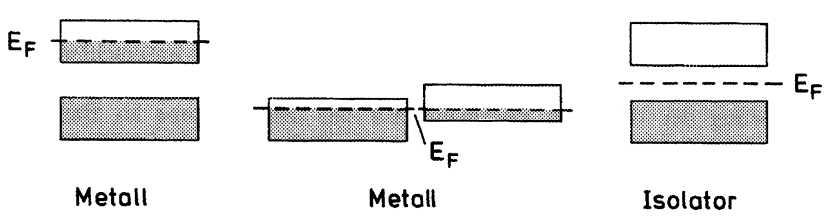
\includegraphics[width=0.8\textwidth]{bilder/bandstruktur.png}    
    \caption{Schematische Darstellung der Bandstrukturen von Metallen(Leitern), Halbleiterm und Isolatoren. Die gestrichelte Linie kennzeichnet die größtmögliche Energie eines Elektrons im Festkörper bei einer Temperatur $T = \SI{0}{\kelvin}$. 
    Diese Energie ist auch als Fermienergie $E_F$ bekannt. Darstellung nach \cite{Kopitzki2017}.}
    \label{fig:bandstruktur}
\end{figure}

\subsection{Dotierung von Halbleitern}
Im folgenden Versuch wird eine n-dotierte 
Galliumarsenidprobe untersucht. Eine n-Dotierung beschreibt das Einbringen eines Fremdatoms in den Halbleiter, welche jeweils ein zusätzliches Valenzelektron besitzen. Diese
zusätzlichen Valenzelektronen sind nun deutlich schwächer gebunden und somit besitzen die Donatorzustände nur eine kleine Bandlücke zum Leitungsband. Je nach Halbleiter und Dotierungsatom sind
diese Bandlücken nur noch einige Millielektronenvolt groß. Sie sind so auch bei Raumtemperatur leitend.
\\
Eine weitere Dotierungsmöglichkeit ist die p-Dotierung. Hierbei werden Fremdatome mit jeweils einem Valenzelektron weniger in den Festkörper gebracht. Es liegt also im Vergleich zum vorherigen Atom eine Elektronenfehlstelle vor. 
Diese Fehlstelle kann nun von anderen Valenzelektron gefüllt werden. Die Löcher können also ab einer gewissen Energie durch den Festkörper wandern. Dieser Prozess wird Löcherleitung genannt.

\subsection{Effektive Masse}

Die effektive Masse stellt ein Hilfsmittel zur Beschreibung von Elektronen oder auch Elektronen-Loch-Paaren in Gittern dar. Diese bewegen sich in einem Kristall
innerhalb des gesamten Gitterpotentials welches nur schwer zu beschreiben und damit zu rechnen ist. Viel einfacher ist eine Betrachtung von freien Teilchen wobei
die Dispersionsrelation
\begin{equation}
E(\vec{k}) = \frac{\hbar^2 \vec{k}^2}{2m}
\end{equation}
bekannt ist. Damit diese Beziehung auch für quasifreie Teilchen gilt, muss die Masse angepasst werden. Bezeichnet wird diese
als effektive Masse $m^*$. Diese lässt sich durch die doppelte Ableitung aus der Energie extrahieren. Für ein eindimensionales Gitter mit ist dies leicht, da
sich die Wellenzahl auf einen Skalar reduziert und es ergibt sich
\begin{equation*}
m^* = \hbar^2 \left( \frac{\partial^2 E(k)}{\partial k^2} \right)^{-1}.
\end{equation*}
Im Allgemeinen muss dies nicht nur auf drei Dimensionen erweitert, sondern es muss auch die Symmetrie und somit die Struktur des Kristalls berücksichtigt werden.
Wenn der Wellenvektor $k_N$ Elemente besitzt dann lässt sich die effektive Masse als 
\begin{equation}
    (m^*)_{ij} = \hbar^2 \left( \frac{\partial^2 E(\vec{k})}{\partial k_i \partial k_j} \right)^{-1}. 
\end{equation}
angeben, also als Tensor welcher durch eine Matrix mit $N \times N$ Einträgen dargestellt werden kann.

\subsection{Zirkulare Doppelbrechung}

Unter zirkularer Doppelbrechung wird die Drehung der Polarisationsrichtung einer linear polarisierten Welle durch einen Kristall verstanden. 
Im folgenden wird erläutert wie sich dies durch Superposition von links- und rechtszirkularen Wellen beschreiben lässt.
\\
Eine zirkualare Welle beschreibt eine in transversal zur Propagationsrichtung schwingende Welle. Wobei eine Komponente um $\pm \pi$/2 phasenverschoben ist.
Daraus ergeben sich folgende Darstellungsmöglichkeiten für links- und rechtszirkulare Wellen
\begin{align*}
E_l &= (E_0 \hat{x} + i E_0 \hat{y}) e^{ik_l z}, \\
E_r &= (E_0 \hat{x} - i E_0 \hat{y}) e^{ik_r z}.
\end{align*}
Hier wurde als mögliche Ausbreitungsrichtung die $z$-Richtung gewählt. Leicht zu erkennen ist, dass bei gleicher Phasengeschwindigkeit, also gleicher Wellenzahl $k_r = k_l$, bei Superposition eine lineare Welle entsteht.
Es lässt sich also schreiben
\begin{equation*}
E(z) = \frac{1}{2} (E_l + E_r).
\end{equation*}
Bei Eintritt in einen Kristall beispielsweise, können durch die Gitterstrukturen die Phasengeschwindigkeit der links- und rechtszirkularen Wellen
voneinander unterscheiden. Sei die Durchlaufslänge der Welle durch den Kristall $L$, so ergibt sich bei $z=L$
\begin{equation*}
    E(L) = E_0 e^{i \phi} (\text{cos}(\theta)\hat{x} + \text{sin}(\theta) \hat{y} ) \quad \text{mit} \quad \theta := \frac{L}{2} (k_r - k_l) \text{ , } \phi := \frac{L}{2} (k_r + k_l).
\end{equation*}
Also resultiert eine um $\theta$ gedrehte lineare Polarisationsrichtung. Gezeigt wurde also, dass eine linear polarisierte Welle, ausgedrückt durch links- und 
rechtszirkulare Wellen, welche in einem Medium zwei
unterschiedliche Phasengeschwindigkeit besitzen, seine Polarisationsrichtung ändert.
Darauf aufbauend lässt sich nun eine makroskopische Erklärung finden.

\subsection{Zirkulare Doppelbrechung durch Polarisation}
In einem Festkörper wird die zirkulare Doppelbrechung durch viele elektrische Dipolmomente hervorgerufen. Diese bilden sich zwischen den Bandelektronen
und den Gitteratomen durch der in dem Festkörper propagierenden Welle aus.
Die makroskopische Polarisation eines Kristalls beschreibt die Summer aller Dipolmomente pro Volumeneinheit und lässt sich beschreiben durch
\begin{equation}
\vec{P} = \epsilon_0 \chi \vec{E}.
\end{equation}
Dabei beschreibt das $\chi$ die dielektrische Suszeptibilität und sie hängt maßgeblich von dem vorliegenden Kristall, nicht nur im Wert, sondern auch in der Form ab.
Bei einem isotropen Kristall reduziert sich die Suszeptibilität auf ein Skalar. Im Allgemeinen ist diese aber ein Tensor, wodurch sich die Gleichung ... auch in Matrixschreibweise formulieren lässt
\begin{equation}
\begin{pmatrix}
P_x \\
P_y \\
P_z 
\end{pmatrix} = 
\begin{pmatrix}
\chi_{xx} & \chi_{xy} & \chi_{xz} \\
\chi_{yx} & \chi_{yy} & \chi_{yz} \\
\chi_{zx} & \chi_{zy} & \chi_{zz}
\end{pmatrix}
\cdot 
\begin{pmatrix}
E_x \\
E_y \\
E_z 
\end{pmatrix}
\end{equation}
In einem Festörper mit makroskopischer Polarisation werden die Maxellgleichungen nun über die dielektrische Verschiebung bestimmt. 
Dabei gilt
\begin{equation}
\vec{D} = \epsilon_o \vec{E} + \vec{P}.
\end{equation}
Für einen Ansatz der dielektrischen Suszeptibilität kann die Wellengleichung nun gelöst werden und es zeigt sich, dass dieser Ansatz
\begin{equation}
    \tilde{\chi} = \begin{pmatrix}
        \chi_{xx} & i\chi_{xy} & 0 \\
        -i\chi_{xy} & \chi_{xx} & 0 \\
        0 & 0 & \chi_{zz}
        \end{pmatrix}
\end{equation}
die Transversalität der Welle wahrt und zwei Lösungen mit
\begin{align*}
    k_+ &= \frac{\omega}{c} \sqrt{(1+\chi_{xx})+ \chi_{xy}} \quad \to \quad v_{\text{ph,r}} = \frac{c}{\sqrt{(1+\chi_{xx})+ \chi_{xy}}}, \\
    k_- &= \frac{\omega}{c} \sqrt{(1+\chi_{xx})- \chi_{xy}} \quad \to \quad v_{\text{ph,l}} = \frac{c}{\sqrt{(1+\chi_{xx})- \chi_{xy}}}.\\
\end{align*}
liefert. Daraus folgt also, dass die Lösungen verschiedene Phasengeschwindigkeiten haben.
Außerdem entstehen die folgenden Zusammenhänge der Feldkomponenten
\begin{equation*}
    E_x = i E_y \quad \text{für } k_+ \quad \quad E_x = -i E_y \quad \text{für } k_-
\end{equation*}
Diese weisen die gleiche Form auf, wie die in Gleichung ... und da die Wellengleichung stets linear ist, ist auch eine Superposition der $k_+$ und $k_-$ Lösungen 
eine Lösung der Gleichung. Gezeigt wurde also, dass es bei einem Festörper mit einer dielektrischen Suszeptibilität der Form ...., zu einer Drehung der Polarisationsrichtung
kommt.

\subsection{Faraday-Effekt}
Bisher wurde nur die Polarisationsänderung bei optisch aktiven Medien gezeigt. Nun lässt sich zeigen, dass diese Drehung ebenfalls bei Anlegen eins magnetischen Feldes parallel in Ausbreitungsrichtung der Welle,
an optisch inaktive Medien geschieht. 
Die Abbildung \ref{fig:drehungitin} zeigt eine solche Drehung bei einem Magnetfeld parallel zu $\vec{z_0}$.
\begin{figure}
    \centering
    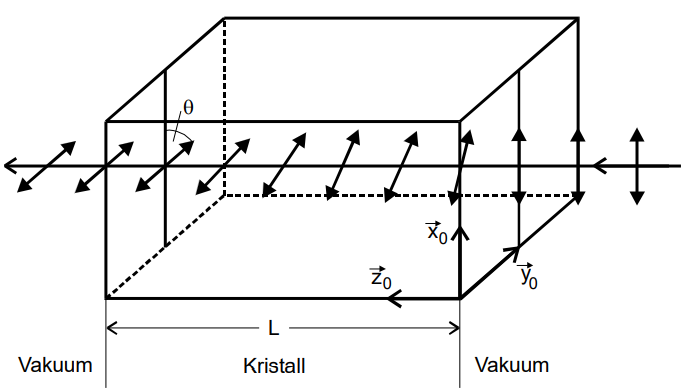
\includegraphics[width=0.8\textwidth]{bilder/drehung.png}    
    \caption{Schematische Darstellung der Faraday-Rotation an einem Kristall. Dabei ist das Magnetfeld parallel zur $\vec{z_0}$ Richtung ausgerichtet. 
    Abbildung nach \cite{skriptanhang}.}
    \label{fig:drehungitin}
\end{figure}
Durch die zuvor dargelegte dielektrische Suszeptibilität lässt sich ein optisch inaktives Medium durch vollständig verschwindende
nicht Diagonalelemente, also $\chi_{ij} = 0 \text{ für }i \neq k$, beschreiben.
\\
In dem Fall eines angeschalteten B-Feldes verhalten sich die Elektronen in den Bändern des Festkörpers anders. Auf sie wirkt nun zusätzlich die Lorentzkraft.
Es lässt sich eine Bewegungsgleichung für die Elektronen aufstellen, unter der Annahme einer Bindung der Elektronen durch ein harmonisches Potential mit Bindungskonstante
$K$. Die Bewegungsgleichung nimmt die folgende Form an 
\begin{equation}
\underbrace{m \frac{\text{d}^2\vec{r}}{\text{d}t^2}}_{\text{Newton}} + \underbrace{K\vec{r}}_{\text{Bindung}} = \underbrace{-e \vec{E}}_{\text{Coulomb}} - \underbrace{-e \frac{\text{d}\vec{r}}{\text{d}t} \times \vec{B}}_{\text{Lorentz}}.
\end{equation}
Das $\vec{r}$ beschreibt die Auslenkung eines Elektrons aus seiner Gleichgewichtslage. In einem klassischen Wellenansatz steckt die zeitabhängigkeit lediglich in einem Phasenfaktor
$\vec{r} \propto \text{exp}(i\omega t)$, wodurch sich die Differentialgleichung vereinfachen lässt.
Außerdem geht mit der Verschiebung $\vec{r}$ auch eine Polarisation einher. Diese ist proportional zur Anzahl der Elektronen pro Volumeneinheit $N$
\begin{equation}
\vec{P} = - e N\vec{r}.
\end{equation}
Dies kann nun genutzt werden, um die Differentialgleichung zu lösen. Hierbei muss wieder ein Ansatz für die Suszeptibilität gemacht werden. Diagonalemente sind nötig, für die Existenz
einer nicht-trivialen Lösung, und die nicht Diagonalelemente müssen rein imaginär sein, damit diese Komponenten nicht von den Feldstärken abhängen, denn dann wären sie bereits ohne 
magnetisches Feld doppelbrechend.
Ein möglicher Ansatz sieht folgendermaßen aus 
\begin{equation}
    \tilde{\chi} = \begin{pmatrix}
        \chi_{xx} & i\chi_{xy} & 0 \\
        i\chi_{yx} & \chi_{xx} & 0 \\
        0 & 0 & \chi_{zz}
        \end{pmatrix}.
\end{equation}
Die Lösung der Differentialgleichung liefert die Bedingung $\chi_{xy} = -\chi_{yx}$, wodurch dieselbe Form wie in ... hergestellt wurde.
Diese durch das B-Feld entstehende Drehung der Polarisationsrichtung wird Faraday-Effekt genannt.
Der Drehwinkel ergibt sich zu
\begin{equation}
\theta = \frac{e^3}{2 \epsilon_0 c} \frac{\omega^2}{(K - \omega^2 m)^2 - (e\omega B)^2} \frac{NBL}{n}.
\end{equation}
Wie bei einem klassischen harmonischen Oszillator lässt sich noch eine Resonanzfrequenz $\omega_0$ definieren, sowie auch eine Zyklotronfrequenz $\omega_c$ als
\begin{align}
\omega_0 &= \sqrt{\frac{K}{m}}, \\
\omega_c &= \frac{e}{m}B.
\end{align}
Die Zyklotronfrequenz ist bei Magnetfeldern von $B \approx \SI{1}{\tesla}$ bei Größenordnungen von $10^{11}\si{\hertz}$, wobei die Resonanzfrequenz, sowie die verwendete Frequenz im
Infrarotbereich $10^{14}$ - $10^{15}\si{\hertz}$ liegt. Die Näherung $(\omega^2_0 \omega^2)^2 >> \omega^2\omega^2_c$ liefert nun
\begin{equation*}
    \theta \approx \frac{e^3}{2 \epsilon_0 c m^2} \frac{\omega^2}{(\omega^2_0 -\omega^2)^2} \frac{NBL}{n}.
\end{equation*}
Nun lässt sich noch der Fall quasifreier Ladungsträger betrachten. Dazu kann $\omega_0 \to 0$ angenommen werden. Zusätzlich lässt sich die Frequenz $\omega$ durch die Wellenlänge $\lambda$ ausdrücken
\begin{equation}
    \theta \approx \frac{e^3}{8 \pi^2 \epsilon_0 c^3 m^2} \lambda^2 \frac{NBL}{n}.
\end{equation}
Damit diese Gleichung trotz leichter Bindung der Leitungselektronen gilt, wird hier die Masse $m$ mit der effektiven Masse $m^*$ ersetzt. Außerdem ist es sinnvoll
den Winkel $\theta$ auf die Probenlänge $L$ zu normieren, wodurch folgt
\begin{equation}
    \theta \approx \frac{e^3}{8 \pi^2 \epsilon_0 c^3 {m^*}^2} \lambda^2 \frac{NB}{n}.
\end{equation}
Anhand dieses Verhältnisses lässt sich also die effektive Masse eines Kristalls am Faraday-Effekt bestimmen.